% Adapted from: http://web.mit.edu/rsi/www/pdfs/beamer-tutorial.tex
\documentclass[pdf]{beamer}
\mode<presentation>{\usetheme{Frankfurt} \useoutertheme{split}}
%\mode<handout>{\usecolortheme{seagull}}
%\usepackage{rsislidepacks}
\usepackage{listings}
\lstset{
  basicstyle=\small,
  columns=fullflexible,
  frame=single,
  breaklines=true,
  postbreak=\mbox{\textcolor{red}{$\hookrightarrow$}\space},
  showstringspaces=false,
}
\usepackage{xcolor}
\usepackage{amsfonts}
\usepackage{amsmath}
\usepackage{amssymb}
\usepackage{amsthm}
\usepackage{graphicx}
\usepackage{url}
\usepackage{pgfplots}
\usetikzlibrary{spy}
%

\usepackage{colortbl}
\usepackage{epstopdf}
\usenavigationsymbolstemplate{}
% title information
\title{Cloud and Big Data}
\subtitle{Big Data Overview}
\author{Gaurav Parashar}
\begin{document}
\begin{frame}
	\thispagestyle{empty}
	\titlepage
\end{frame}
\addtocounter{framenumber}{-1}
\tableofcontents

%%%%%%%%%%%%%%%%%%%%%%%%%%%%%%%%%%%%%%%%
\section{Objectives}
\begin{frame}{Objectives}
	\begin{itemize}
		\item Understand Big Data? \pause
		\item Application areas of Big Data \pause
		\item Analyse limitations of existing systems \pause
		\item Big Data Analytics in Industry Verticals \pause
		\item Understand Hadoop and its features \pause
		\item How to configure Virtual Machine \pause
		\item Perform read and write in Hadoop \pause
		\item Understand what is Cloud?\pause
		\item How to configure Cloud Environment? \pause
		\item How to perform operations on Big Data in Cloud Environment
	\end{itemize}
\end{frame}


\section{Introduction}

%%%%%%%%%%%%%%%%%%%%%%%%
\subsection{What does "Big Data" Mean?}

\begin{frame}{What does "Big Data" Mean?}
	\begin{itemize}
		\pause
		\item Collecting large amounts of data
		\pause
		\begin{itemize}
			\item Computers, Databases, Video, Voice , tweets, comments, blogs, web pages, logs, calls, messages (Text + Whatsapp + ...) ,...
		\end{itemize}
	\end{itemize}
\pause
 What do we do with this data?	
\begin{itemize}
		\pause
		\item Early Fraud Detection, Credit Card Frauds, Tick~\cite{tic} Analytics 
		\pause
		\item Content personalisation, Recommendation System  
		\pause
		\item Insurance: Personalised Pricing
		\pause
		\item Customer Loyalty Data
		\pause
		\item Predicting Future
	\end{itemize}
\end{frame}
\subsection{Applications of Big Data}
\begin{frame}[fragile]{Applications of Big Data}
Examples: \\
Google Trends
	 \begin{figure}[ht]
	    \begin{center}
        		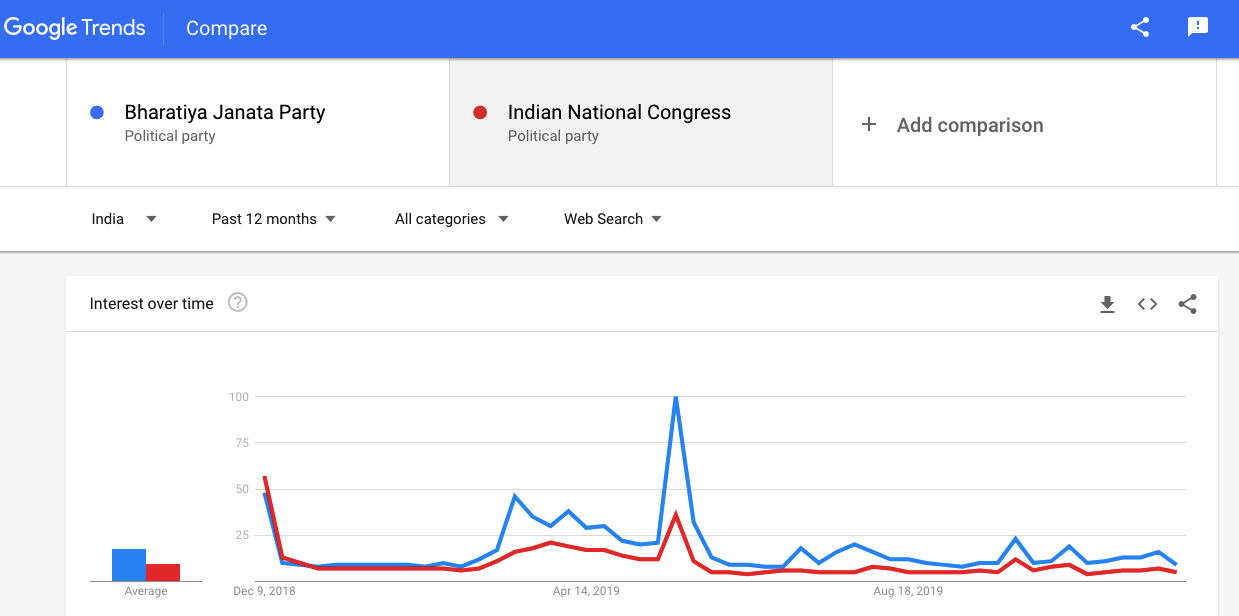
\includegraphics[height=2in]{1.png}
            ~\footnote{Google Trends for BJP and INC}
    \end{center}
    \end{figure}
\end{frame}
\begin{frame}[fragile]{Applications of Big Data}
Maps
	 \begin{figure}[ht]
	    \begin{center}
        		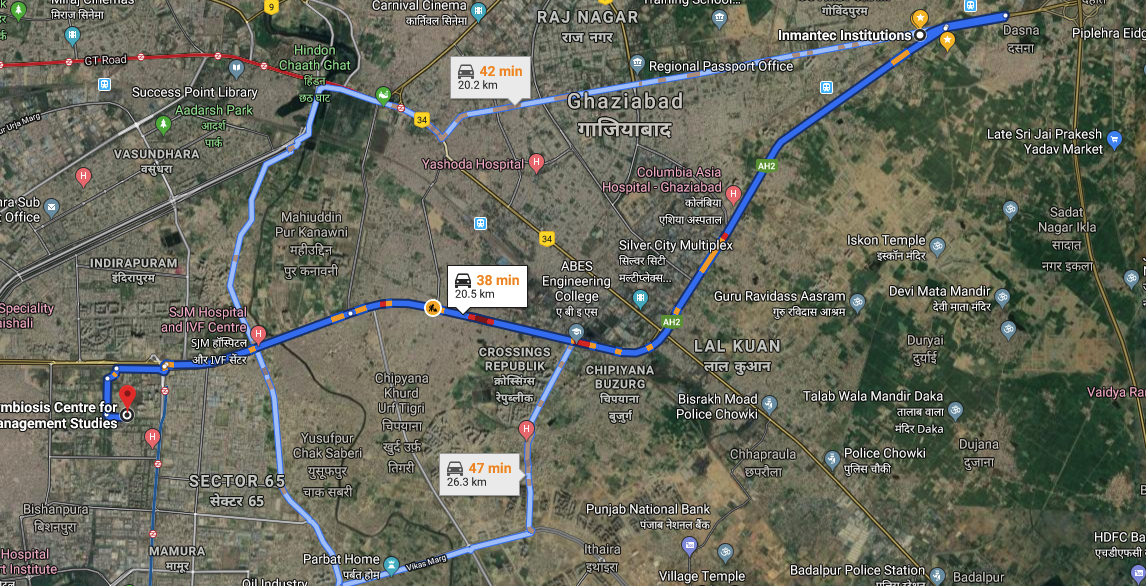
\includegraphics[height=2.2in]{2.png}
            ~\footnote{Display path, traffic, terrain, etd. time}
    \end{center}
    \end{figure}
\end{frame}

\begin{frame}[fragile]{Applications of Big Data}
Recommendation Systems
	 \begin{figure}[ht]
	    \begin{center}
        		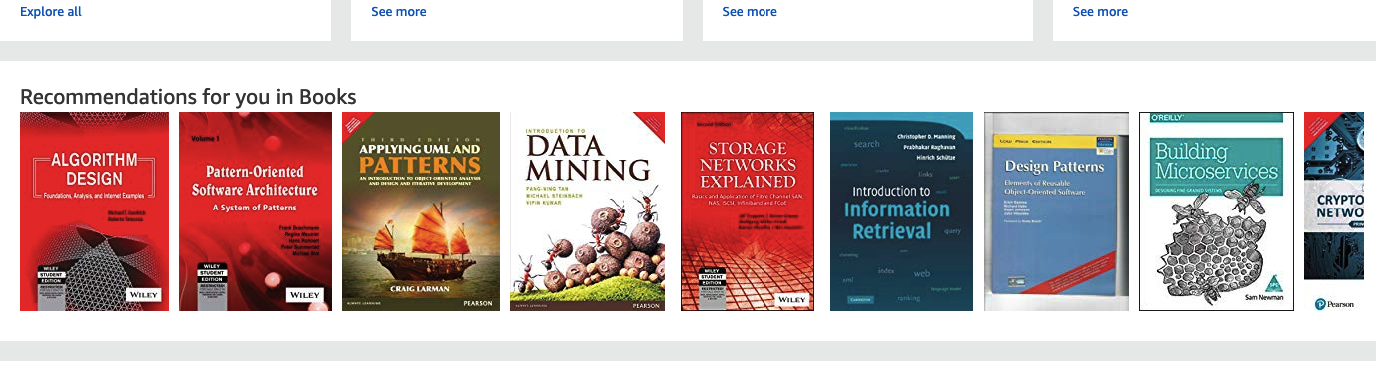
\includegraphics[height=2.2in]{3.png}
            ~\footnote{Recommendation Engine}
    \end{center}
    \end{figure}
\end{frame}

\begin{frame}[fragile]{Applications of Big Data}
Twitter Trends
	 \begin{figure}[ht]
	    \begin{center}
        		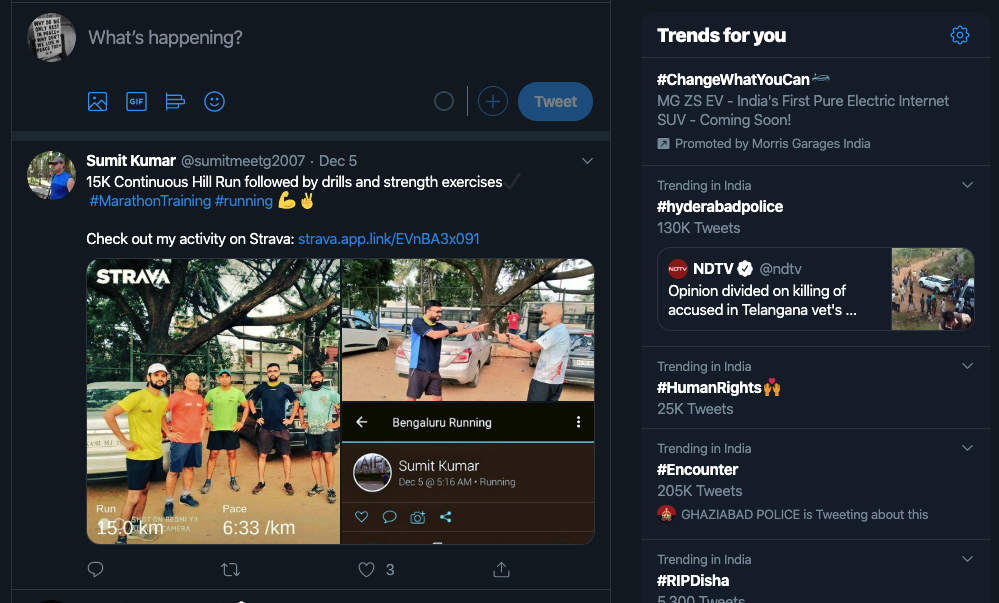
\includegraphics[height=2in]{4.png}
            ~\footnote{Trending in Twitter}
    \end{center}
    \end{figure}
\end{frame}

\begin{frame}[fragile]{Applications of Big Data}
Big Data in Sports~\cite{GudmundssonH16}
	 \begin{figure}[ht]
	    \begin{center}
        		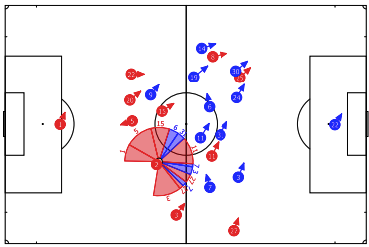
\includegraphics[height=2in]{6.png}
		\caption{Available receivers of pass by Red2}
            ~\footnote{Spatio-Temporal Analysis of Team Sports - {A} Survey}
    \end{center}
    \end{figure}
\end{frame}
\begin{frame}[fragile]{Applications of Big Data}
\begin{itemize}
    \item Weather Prediction
    \item Medical Diagnosis
    \item Smart Cities and Buildings
 \end{itemize}	
\end{frame}

\subsection[Generation of Big Data]{Generation of Big Data}
\begin{frame}[fragile]{Generation of Big Data}
	 \begin{figure}[ht]
	    \begin{center}
        		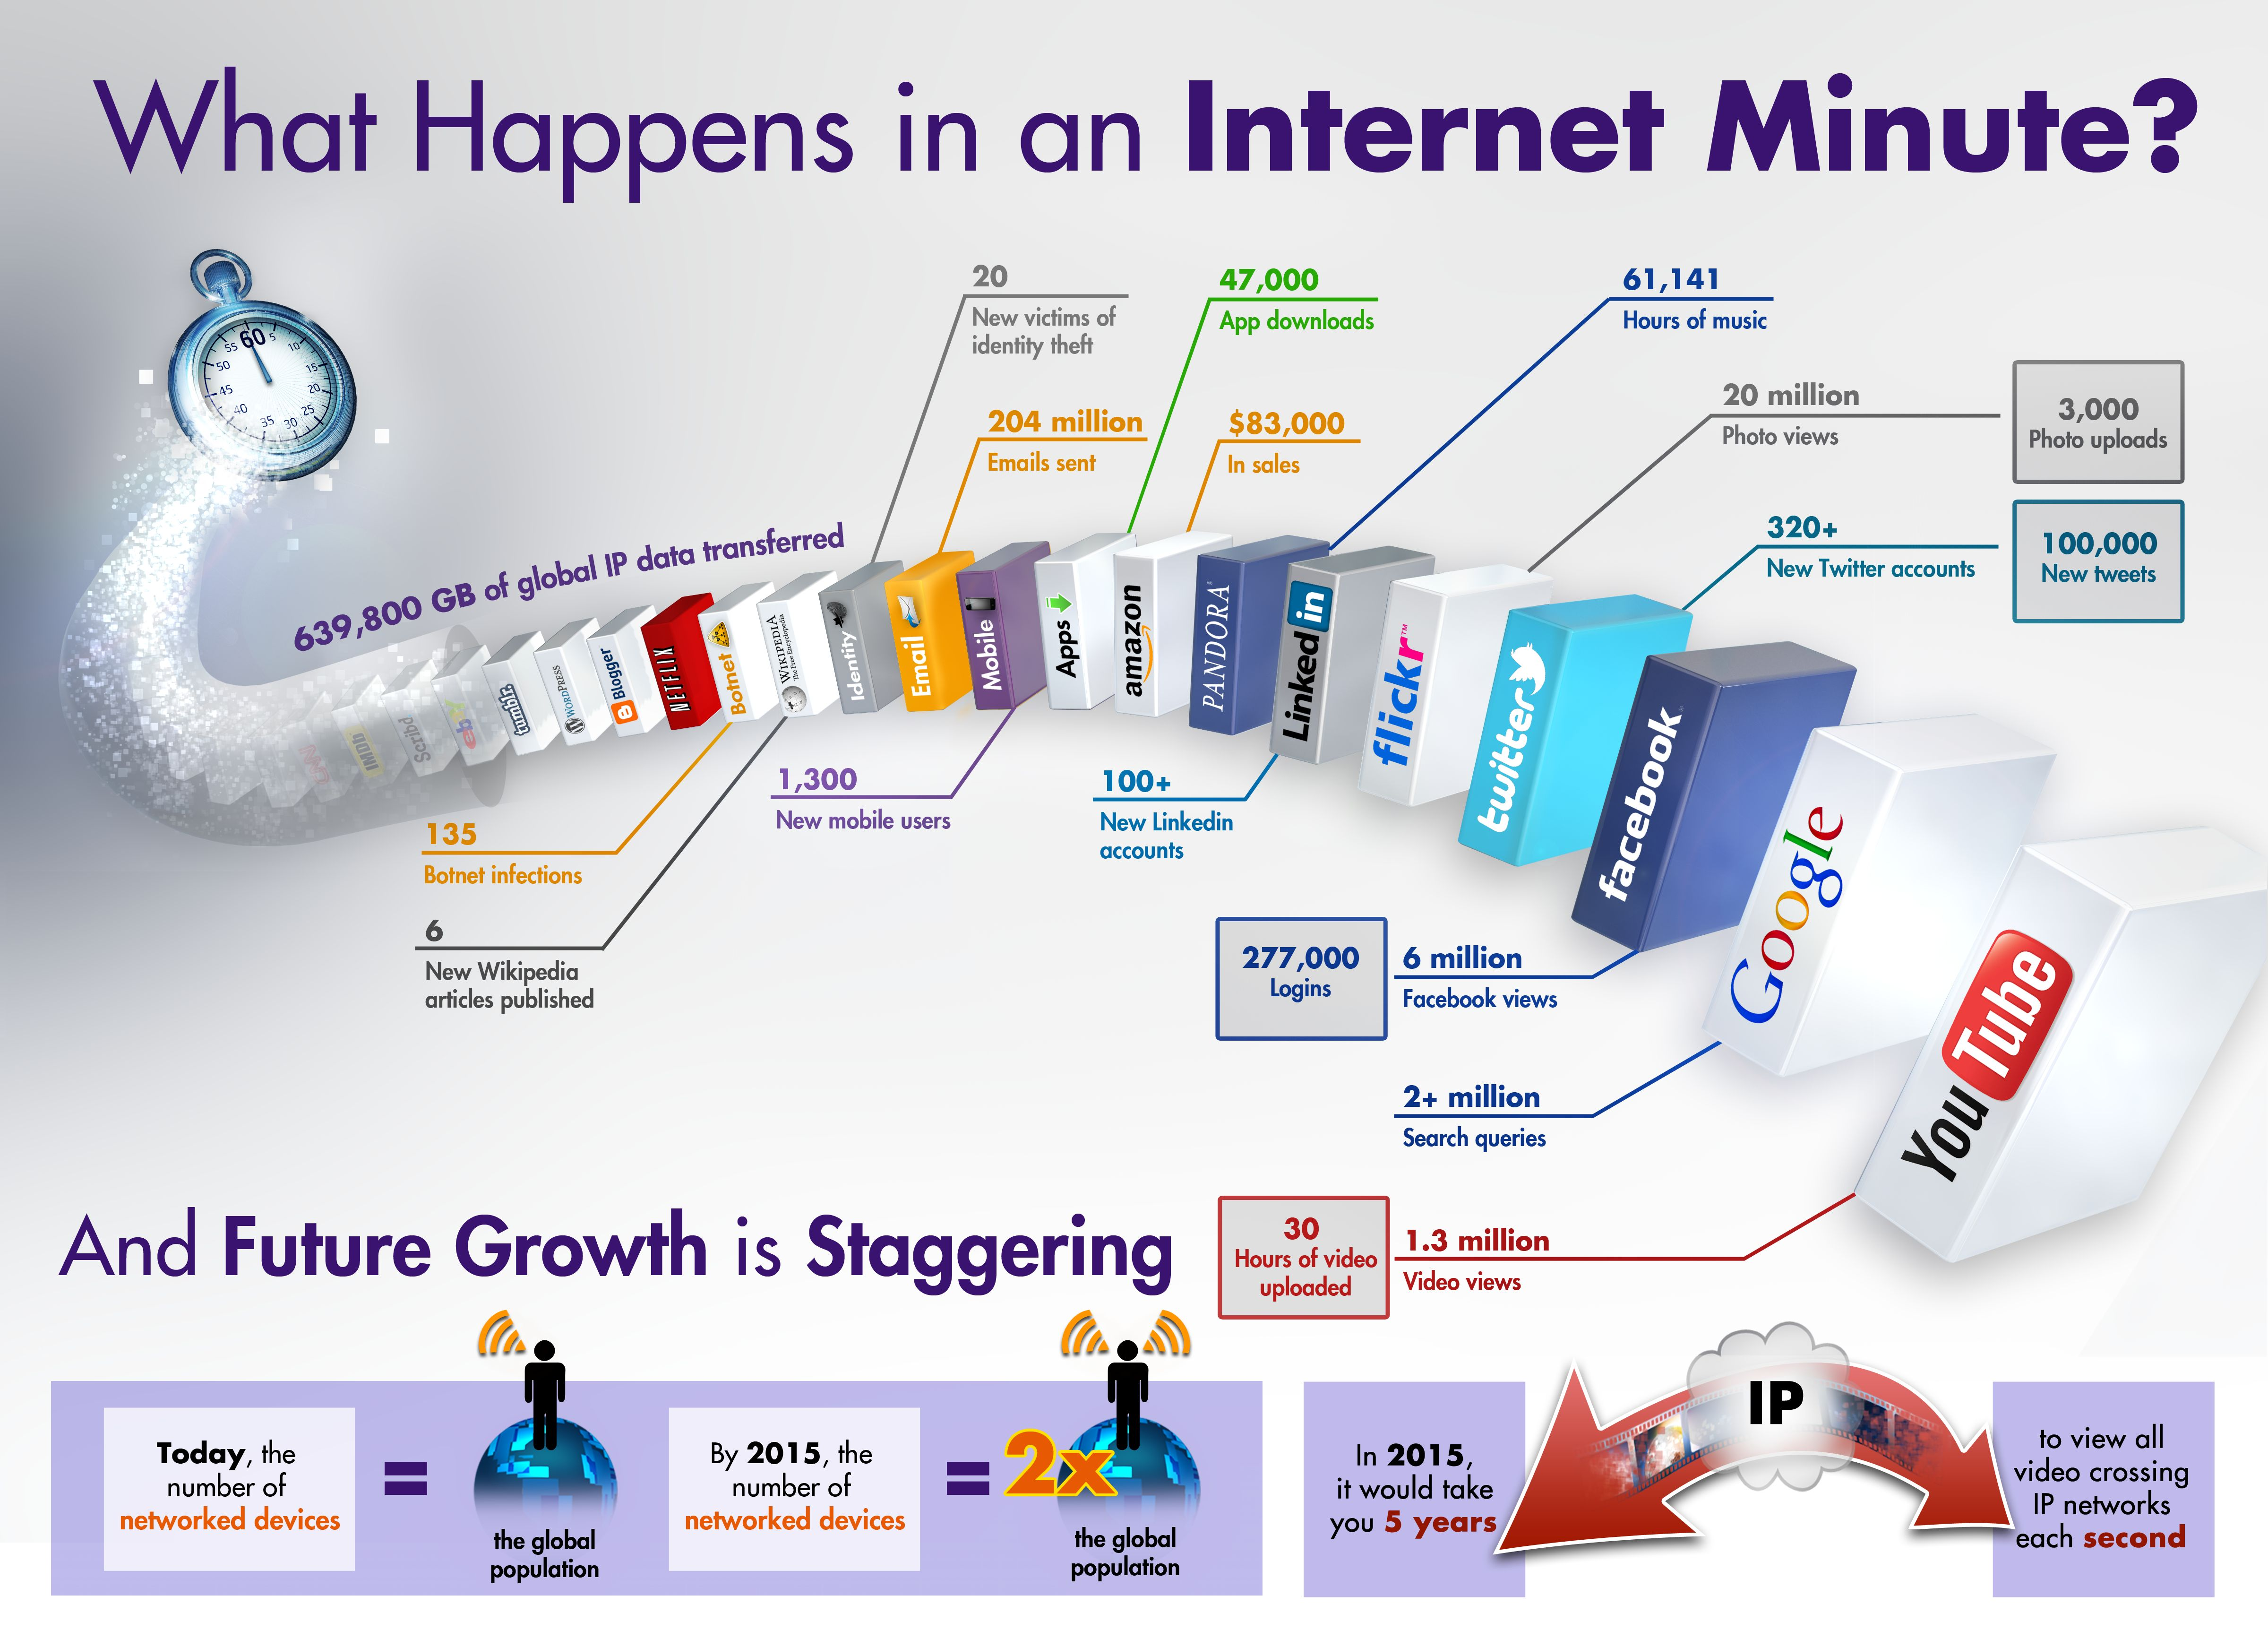
\includegraphics[height=2.9in]{5.jpg}
    \end{center}
    \end{figure}
\end{frame}

\section[6 Vs of Big Data]{6 Vs of Big Data}
%%%%%%%%%%%%%%%%%%%%%%%%%
%			Volume					%
%%%%%%%%%%%%%%%%%%%%%%%%%
\begin{frame}[fragile, label={vol}]{6 Vs of Big Data\cite{5vs}: Volume~\ref{iv1}}
\begin{tikzpicture}[spy using outlines ={magnification=2, circle, size=5cm, red, connect spies}]
\node (h1) at (0,0) {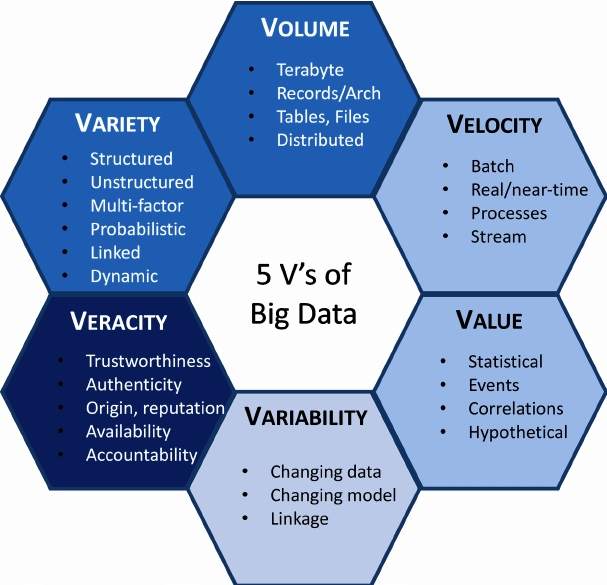
\includegraphics[height=2.9in]{7.png}};
\spy on (0.2,2.5)  in node at (6,1); 
\end{tikzpicture}
\end{frame}

\begin{frame}[fragile]{Scenario: Volume}
What is the staring limit of Big Data?
\begin{enumerate}[A]
\item $>$ 1 GB - $<$ 1TB \pause
\item  $>$ 1 TB - $<$ 1PB\pause
\item $>$ 1 PB - $<$ 1EB\pause
\item $>$ 1 EB - $<$ 1ZB\pause
\end{enumerate}
\uncover {Answer:}\\
\uncover {\small{Depends upon the organisation definition of Big Data. Relative term.}}

\end{frame}

\begin{frame}[fragile]{Scenario: Volume~\ref{iv1}}
 \begin{figure}[ht]
	    \begin{center}
        		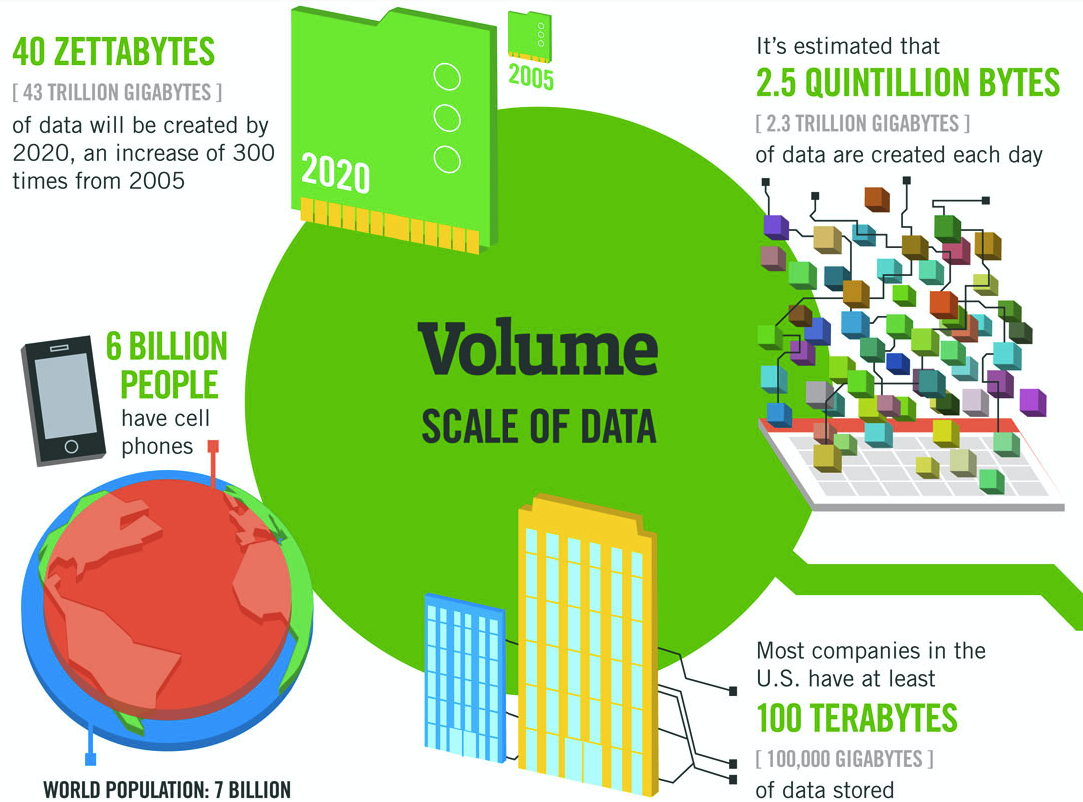
\includegraphics[height=2.7in]{9.png}
    \end{center}
    \end{figure}
\end{frame}

%%%%%%%%%%%%%%%%%%%%%%%%%
%			Velocity					%
%%%%%%%%%%%%%%%%%%%%%%%%%
\begin{frame}[fragile, label={vel}]{6 Vs of Big Data: Velocity~\ref{iv1}}
\begin{tikzpicture}[spy using outlines ={magnification=1.7, circle, size=4.5cm, red, connect spies}]
\node (h1) at (0,0) {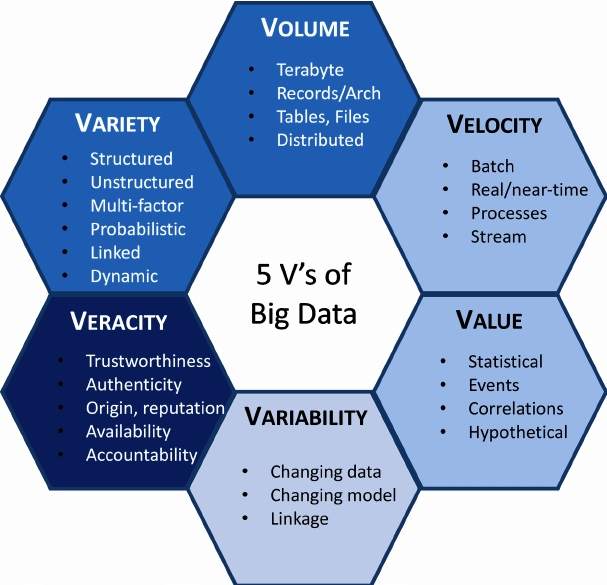
\includegraphics[height=2.9in]{7.png}};
\spy[thick, size=5cm] on (2.6,1.5)  in node at (6,-0.7); 
\end{tikzpicture}
\end{frame}


\begin{frame}[fragile]{6 Vs of Big Data: Velocity}
\begin{figure}[ht]
	    \begin{center}
        		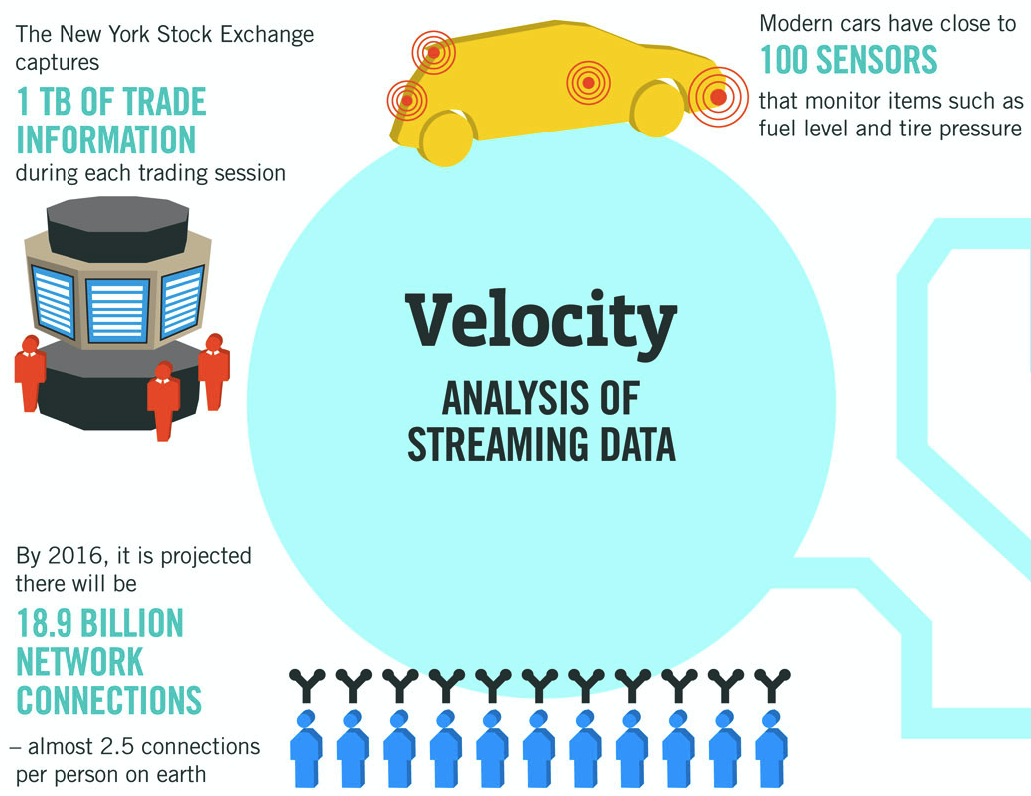
\includegraphics[height=2.7in]{8.png}
    \end{center}
    \end{figure}
\end{frame}
%%%%%%%%%%%%%%%%%%%%%%%%%
%			Value					%
%%%%%%%%%%%%%%%%%%%%%%%%%
\begin{frame}[fragile, label={val}]{6 Vs of Big Data: Value~\ref{iv1}}
\begin{tikzpicture}[spy using outlines ={magnification=2, circle, size=4.5cm, red, connect spies}]
\node (h1) at (0,0) {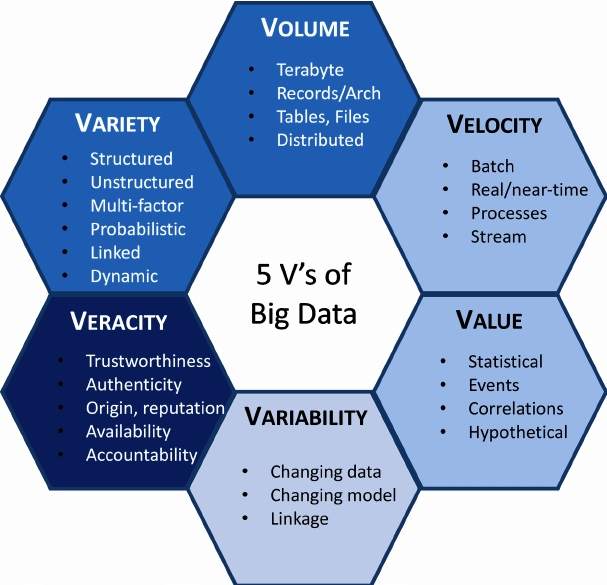
\includegraphics[height=2.9in]{7.png}};
\spy[thick, size=5cm] on (2.5,-1.2)  in node at (6,1.7); 
\end{tikzpicture}
\end{frame}

%%%%%%%%%%%%%%%%%%%%%%%%%
%			Variability					%
%%%%%%%%%%%%%%%%%%%%%%%%%
\begin{frame}[fragile, label={var}]{6 Vs of Big Data: Variability~\ref{iv1}}
\begin{tikzpicture}[spy using outlines ={magnification=2, circle, size=5cm, red, connect spies}]
\node (h1) at (0,0) {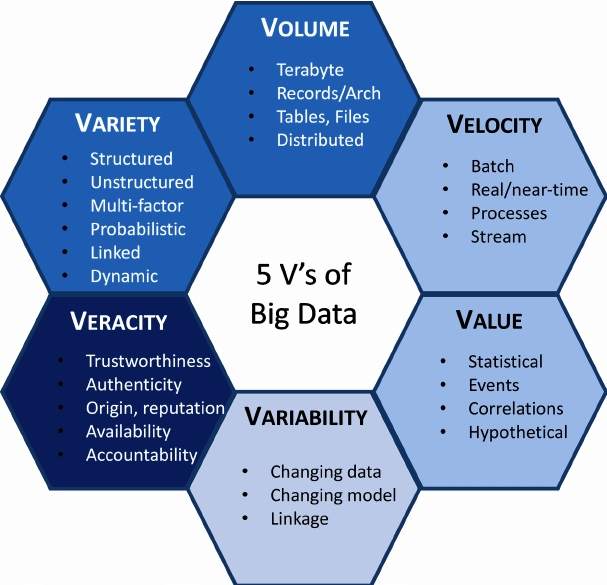
\includegraphics[height=2.9in]{7.png}};
\spy[thick, size=5cm] on (0.2,-2.2)  in node at (6.1,1.7); 
\end{tikzpicture}
\end{frame}

%%%%%%%%%%%%%%%%%%%%%%%%%
%			Veracity					%
%%%%%%%%%%%%%%%%%%%%%%%%%
\begin{frame}[fragile, label={ver}]{6 Vs of Big Data: Veracity~\ref{iv1}}
\begin{tikzpicture}[spy using outlines ={magnification=2, circle, size=4.5cm, red, connect spies}]
\node (h1) at (0,0) {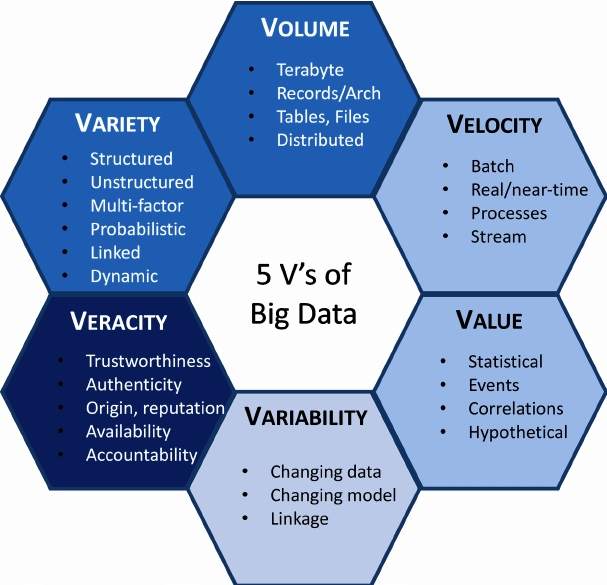
\includegraphics[height=2.9in]{7.png}};
\spy[thick, size=5.5cm] on (-2.1,-1.2)  in node at (5,1.7); 
\end{tikzpicture}
\end{frame}

%%%%%%%%%%%%%%%%%%%%%%%%%
%			Variety					%
%%%%%%%%%%%%%%%%%%%%%%%%%
\begin{frame}[fragile, label={vari}]{6 Vs of Big Data: Variety~\ref{iv1}}
\begin{tikzpicture}[spy using outlines ={magnification=2, circle, size=4.5cm, red, connect spies}]
\node (h1) at (0,0) {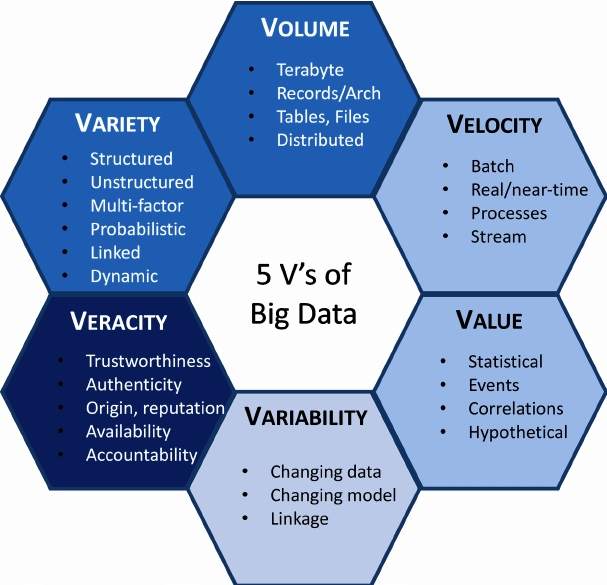
\includegraphics[height=2.9in]{7.png}};
\spy[thick, size=5cm] on (-2.3,1.2)  in node at (5,1.7); 
\end{tikzpicture}
\end{frame}

%%%%%%%%%%%%%%%%%%%%%%%%%
	%	Limitations of Existing Systems	%
%%%%%%%%%%%%%%%%%%%%%%%%%
\subsection{Limitations of Existing Systems}
\begin{frame}[fragile]{Limitations of Existing Systems}
\begin{enumerate}
	\item Cost of scaling \pause
	\item Vertical Scaling \pause
	\item Integration with legacy systems \pause
	\item Rapid Change in type of data \pause
	\item Lack of skills
\end{enumerate}
\end{frame}

%%%%%%%%%%%%%%%%%%%%%%%%%
	%	Industry Verticals	%
%%%%%%%%%%%%%%%%%%%%%%%%%
\section{Application of Big Data in Industry Verticals}
\subsection{ Telecom}
\begin{frame}[allowframebreaks, label={iv1}]{Home Work Question 1:Telecom}
A telco\cite{vtata} serving 8 million prepaid mobile subscribers
\begin{enumerate}
	\item Volume~\ref{vol}: \underline{\hspace{3cm}}
	\item Velocity~\ref{vel}:  \underline{\hspace{3cm}}
	\item Value~\ref{val}: \underline{\hspace{3cm}}
	\item Variability~\ref{var}: \underline{\hspace{3cm}}
	\item Veracity~\ref{ver}:  \underline{\hspace{3cm}}
	\item Variety~\ref{vari}:  \underline{\hspace{3cm}}
\end{enumerate}

Link: https://github.com/gauravparashar/symbiosis

\end{frame}

\subsubsection{Call Detail Record}
\begin{frame}[fragile]{}
\begin{figure}[ht]
	    \begin{center}
        		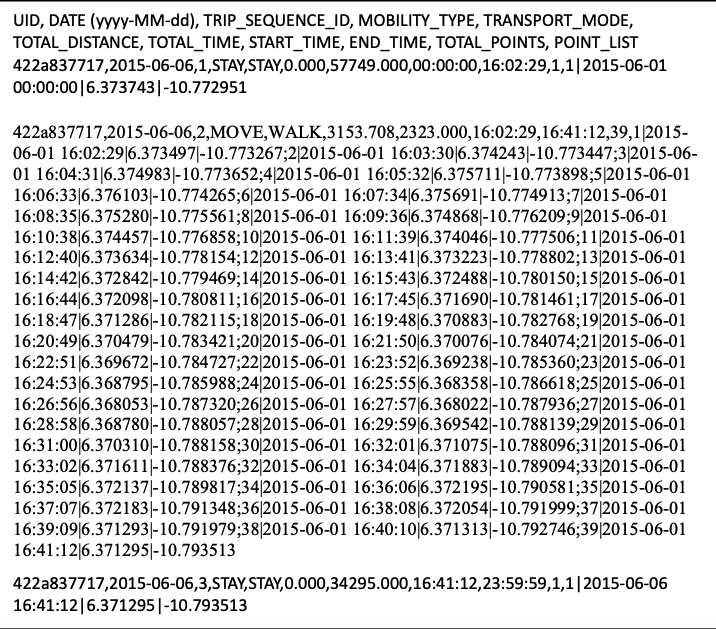
\includegraphics[height=2.8in]{cdr.png}
    \end{center}
    \end{figure}
\end{frame}
%%%%%%%%%%%%%%%%%%%%%%%%%%%%%%%%%%%\
%%%%%%%%%%%%%%%%%%%%%%%%%%%%%%%%%%%
\section{Hadoop HDFS and its features}
\begin{frame}[fragile]{}
Hadoop is a distributed system which is based on HDFS (Hadoop Distributed File System). It is scalable, distributed, and portable file system for large commodity systems. 
\begin{itemize}
	\item stores large amount of data 
	\item reliable way to store data
	\item scalable way to manage resources
	\item HDFS is composed of two main components
	\begin{itemize}
		\item Name Node
		\item Data Node
	\end{itemize}
\end{itemize}
\end{frame}


\subsection{Hadoop Design}
\begin{frame}[fragile]{}
\begin{figure}[ht]
	    \begin{center}
        		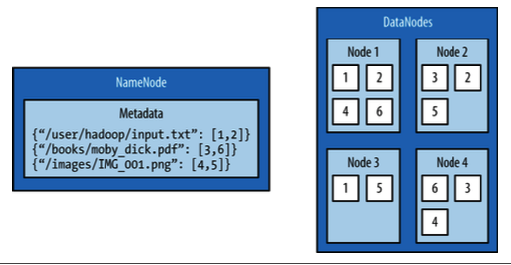
\includegraphics[height=2in]{12.png} \cite{hpy}
    \end{center}
    \caption{HDFS Architecture ~\footnote{HDFS cluster with replication factor of  2}}
    \end{figure}
\end{frame}

\subsection{Interacting with HDFS}
\begin{frame}[fragile]{}
\noindent Interaction with HDFS is primarily performed from the command line using command \textbf{\emph{hdfs}}.
\begin{lstlisting}[language=bash]
  $ hdfs COMMAND [-option <arg>]
\end{lstlisting}
The command argument instructs which functionality of HDFS to be used.

\end{frame}

\section{Interacting with HDFS}
\begin{frame}[fragile]{Common File Operations}
\noindent To perform basic operations on HDFS, we use \textbf{\emph{dfs}} command with \textbf{\emph{hdfs}}.
\textbf{\emph{dfs}} supports many file operations like copy, move, remove , etc. \\
List directory contents
\begin{lstlisting}[language=bash]
  $ hdfs dfs -ls /
\end{lstlisting}
It lists out the content of the root filesystem of HDFS.

\end{frame}
\subsection{List Directory Contents}
\begin{frame}[fragile]{List Directory Contents}
Output: 
\begin{lstlisting}[language=bash]
$ hdfs dfs -ls /
Found 3 items
drwxr-xr-x - hadoop supergroup 0 2019-12-28 23:20 /input
drwxr-xr-x - hadoop supergroup 0 2019-12-29 00:18 /output
drwx------ - hadoop supergroup 0 2019-12-18 22:33 /tmp
\end{lstlisting}

\end{frame}


\subsection{Creating a Directory}
\begin{frame}[fragile]{}
To create a directory within HDFS.
\begin{lstlisting}[language=bash]
$ hdfs dfs -mkdir /user
\end{lstlisting}

Output: 
\begin{lstlisting}[language=bash]
$ hdfs dfs -mkdir /user
Found 4 items
drwxr-xr-x - hadoop supergroup 0 2019-12-28 23:20 /input
drwxr-xr-x - hadoop supergroup 0 2019-12-29 00:18 /output
drwx------ - hadoop supergroup 0 2019-12-18 22:33 /tmp
drwxr-xr-x - hadoop supergroup 0 2020-01-03 22:22 /user
\end{lstlisting}
\end{frame}

\subsection{Copy Data onto HDFS}
\begin{frame}[fragile]{}
Copy data file(s) onto HDFS.
\begin{lstlisting}[language=bash]
$ hdfs dfs -put source destination
\end{lstlisting}

Output: 
\begin{lstlisting}[language=bash]
$ hdfs dfs -put hw.csv /user
\end{lstlisting}
-get command can be used to retrieve data from HDFS to local file system
\end{frame}


\subsection{Display Content of a file from HDFS}
\begin{frame}[fragile]{}
To visualise the content in the file copied onto HDFS
\begin{lstlisting}[language=bash]
$ hdfs dfs -cat filename
\end{lstlisting}
Output: 
\begin{lstlisting}[language=bash]
$ hdfs dfs -cat /user/hw.csv 
1,65.78331,112.9925
2,71.51521,136.4873
3,69.39874,153.0269
4,68.2166,142.3354
....
24999,67.52918,132.2682
25000,68.87761,124.8742
\end{lstlisting}

-head command can be used to display 50 lines from top.
\\
-tail command can be used to display last 50 lines from bottom.
\end{frame}



\section{MapReduce}
\begin{frame}[fragile]{}
MapReduce is a programming model that enables large volumes of data to be processed and generated by dividing work into independent tasks and executing the tasks in parallel across a cluster of machines.

\begin{figure}[ht]
	    \begin{center}
        		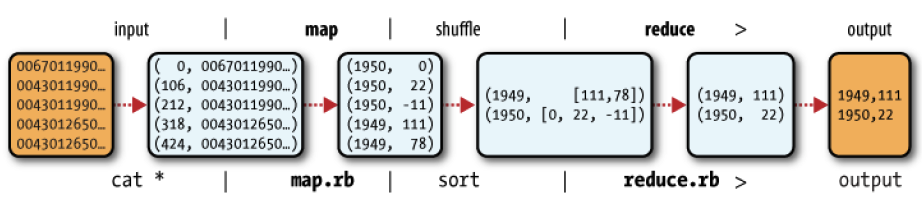
\includegraphics[height=1.1in]{13.png}
    \end{center}
    \caption{MapReduce logical data flow\cite{hdg}}
    \end{figure}
\end{frame}



\section{Python}
\begin{frame}[fragile]{Word Count Example - Prerequisite}
	\begin{itemize}
	\item sys module
	: A file containing a set of functions you want to include in your application.
\begin{lstlisting}[language=python]
import sys
\end{lstlisting}		
	\item for loop
	: A for loop is used for iterating over a sequence (that is either a list, a tuple, a dictionary, a set, or a string).
\begin{lstlisting}[language=python]
students = ["Aman", "Anita", "Cherry"] 
for student in students: 
	print(student)
\end{lstlisting}
	\item  lists : List is a collection which is ordered and changeable. Allows duplicate members
\begin{lstlisting}[language=python]
students = ["Aman", "Anita", "Cherry"] 	
\end{lstlisting}	
	\end{itemize}
\end{frame}

\begin{frame}[fragile]{Word Count Example - Prerequisite}
\begin{itemize}
	\item print : The print() function prints the specified message to the screen, or other standard output device.
\begin{lstlisting}[language=python]
	print "%s\t%s" %("Hello", "how are you?")
	print '{0}\t{1}'.format("Hello", "how are you?")
\end{lstlisting}

	\item split : split(separator) function returns a list of strings after breaking the given string by the specified separator.

\begin{lstlisting}[language=python]
	line = "Mary had alittle lamb"
	print (line.split(" "))
\end{lstlisting}

\end{itemize}		
\end{frame}


\begin{frame}[fragile]{Word Count Example - Prerequisite}
\begin{itemize}
	\item dictionary : Dictionary is an unordered collection of data values, used to store data values like a map, which unlike other Data Types that hold only single value as an element, Dictionary holds key:value pair. 
\begin{lstlisting}[language=python]
# Creating an empty Dictionary 
Dict = {} 
print("Empty Dictionary: ") 
print(Dict) 
  
# Creating a Dictionary with Integer Keys 
Dict = {1: 'Geeks', 2: 'For', 3: 'Geeks'} 
print("\nDictionary with the use of Integer Keys: ") 
print(Dict) 

\end{lstlisting}
\end{itemize}		
\end{frame}



\begin{frame}[fragile]{Python Hadoop: Final Mapper code}
\begin{lstlisting}[language=python]
for line in sys.stdin:
    line =  line.strip() # Remove the leading and trailing spaces
    words =  line.split() # Split the line on space
    for word in words:
         print "%s\t%s" %(word,1) # you can use this method or
         print '{0}\t{1}'.format(word, 1) #this method
\end{lstlisting}
\end{frame}

\begin{frame}[fragile]{Python Hadoop: Final Mapper output}
\begin{lstlisting}[language=bash]
$ echo Hello world. I am an Indian. and I love my country | python mapper.py 
\end{lstlisting}
Output:
\begin{lstlisting}[language=bash]
Hello   1
world.  1
I       1
am      1
an      1
Indian. 1
and     1
I       1
love    1
my      1
country 1
\end{lstlisting}
\end{frame}

\begin{frame}[fragile]{Python Hadoop: Final Reducer code}
\begin{lstlisting}[language=python]
import sys
w = {}
# Process each key-value pair from the mapper
for line in sys.stdin:
    # Get the key and value from the current line
    word, count = line.split('\t')
    # Convert the count to an int
    count = int(count)
    if word in w:
        w[word] = w[word] + count
    else:
        w[word] = count

for word in w.keys():
    print "%s\t%s" %(word,w[word])
\end{lstlisting}
\end{frame}



\begin{frame}[fragile]{Python Hadoop: Final Reducer output}
\begin{lstlisting}[language=bash]
$ echo Hello world. I am an Indian. and I love my country | python mapper.py | python reducer.py
\end{lstlisting}
Output:
\begin{lstlisting}[language=bash]
and     1
love    1
I       2
my      1
am      1
an      1
Indian. 1
country 1
world.  1
Hello   1
\end{lstlisting}
\end{frame}


\begin{frame}[fragile]{Python Hadoop: Final Execution on Hadoop}
\begin{lstlisting}[language=bash]
$ hdfs dfs -put code/first_code/data.txt /input
mapred streaming -input /input/data.txt  -output /output/ -file ~/symbiosis/code/first_code/mapper.py -mapper ~/symbiosis/code/first_code/mapper.py -file ~/symbiosis/code/first_code/reducer.py -reducer ~/symbiosis/code/first_code/reducer.py
\end{lstlisting}
\end{frame}

\begin{frame}[fragile]{Python Hadoop: Final Execution on Hadoop}
\begin{lstlisting}[language=bash]
$ hdfs dfs -ls /output/
Found 2 items
-rw-r--r--   1 hadoop supergroup 0 2020-01-07 11:59 /output/_SUCCESS
-rw-r--r--   1 hadoop supergroup 69 2020-01-07 11:59 /output/part-00000
$hdfs dfs -cat /output/*
and     1
love    1
I       2
country 1
am      1
an      1
Indian. 1
my      1
Hello   1
world.  1
\end{lstlisting}
\end{frame}



%%%%%%%%%%%%%%%%%%%%%%%%
%References
%%%%%%%%%%%%%%%%%%%%%%%%%%%%%%%%%%%%%%%%
\section{References}
\bibliography{biblio} 
\bibliographystyle{ieeetr}
\end{document}
